\documentclass[11pt]{article}
\usepackage{geometry}
\geometry{margin=.94in}
\usepackage[OT1]{fontenc}
\usepackage{booktabs}
\usepackage{adjustbox}
\usepackage[backend=bibtex8,style=authoryear]{biblatex}
\bibliography{lib}
\title{\vspace{-1.5cm}IDS703 Final Project Report}
\author{Anna Dai, Satvik Kishore, Moritz Wilksch}
\date{December 12th, 2021}

\begin{document}
\maketitle

% --------------------------------------------------------------------------------

\section{Introduction}

In this project, we work on tweet classification as a Natural Language Processing problem, more specifically, as a document classification problem. Twitter is a microblogging service where users post publicly visible ``Tweets", which are essentially texts with less than 280 characters. These Tweets may also contain other media objects which are discarded for the purposes of this project. These Tweets most often serve as discussion pieces as part of larger conversations. They are relevant to any number of topics under discussion. These ``topics" are also often explicitly highlighted by the user using a ``hashtag", i.e. text with `\#' followed by the topic name, or a commonly used shorthand for it. For the purpose of our project, we treat these hashtags as ``topics" for our document classification model, where each Tweet is an instance of a document.

% --------------------------------------------------------------------------------
\section{Data}

\subsection{Collection}
We manually select seven popular topics (hashtags) for classification: \texttt{crypto}, \texttt{tesla}, \texttt{championsleague}, \texttt{formula1}, \texttt{thanksgiving}, \texttt{holidays}, and \texttt{covid19}. These topics were intentionally selected so that some topics have some degree of overlap between them (e.g. \texttt{holidays} and \texttt{thanksgiving}), others are easier to differentiate (e.g. \texttt{crypto} vs \texttt{formula1}), and one is an independent topic that is often mentioned with the others (i.e. \texttt{covid19}). We leverage the python library TWINT (\cite{twint}) to scrape approximately 10,000 Tweets, or documents, for each of these seven topics.

\subsection{Pre-Processing}

The raw scraped Tweets are quite messy as they are cluttered with media objects like links, images, mentions of other Twitter users (i.e. @usernames), other hashtags, etc., so we spend some time to carefully pre-process the data before proceeding with modeling. As a first step, we utilize regular expressions (regex) to remove any peripheral content such as URLs, mentions, hashtags, and cashtags. We then normalize our corpus by converting it to lowercase, stripping all punctuation marks, replacing all numbers with ``\textless number\textgreater" with regex and removing stopwords (e.g. and, the, to) using the NLTK stopwords library. Lastly, we tokenize each document into separate words and encode these words using a TorchNLP's WhitespaceEncoder. We specifically choose to retain all emojis as tokens because we believe they have value in topic classification, however, multiple emojis strung together were treated as different tokens, resulting in an artificially inflated corpus. Thus, we leverage the emojis' unicode character codings to break up emojis into unique tokens.
\\[5pt]
\noindent Once cleaned, we randomly split the corpus of 70,000 documents to form our train, validation, and test data sets in a 60/20/20 ratio respectively. We will train models on the train set, find optimal hyperparameters using the validation set, and report all performance metrics in the \emph{Results} section on the test set, which is used only once to evaluate each model.

% --------------------------------------------------------------------------------

\section{Modeling}
\subsection{Generative Model}
We use a Latent Dirichlet Allocation (LDA) model as a generative model to learn from the corpus we have collected. This type of model does not require any hyperparamter tuning, and thus is trained using a combination of the training and validation dataset. We used the LDA implementation from scikit-learn (\cite{sklearn}). It is fit to the corpus to infer seven separate topics, as this is the number of actual topics in the training set. Subsequently, for each inferred topic, we manually inspect the top 50 words that are associated with it in order to assign it a name or label. This manual step is necessary, as the order of topics is not preserved. In fact, the LDA model does not even guarantee to find the same topics that were collected in the original data set. This shortcoming will be discussed in the \emph{Results} and \emph{Conclusion} sections. 
To use the LDA for document classification,  we let the model infer the topic distribution of each document in the test set and use the $argmax(\cdot)$ function to assign each document the topic that is most prevalent according to the LDA.
Finally, the LDA is used to generate synthetic data. For each topic, we sample 10,000 artificial documents, the length of which is sampled from the empirical distribution of tweet lengths each time. Similar to the actual data set, the synthetic data set is also split into a train, validation, and test set using a 60/20/20 ratio split.


\subsection{Discriminative Model}
We develop a neural network model as a discriminative model in order to classify input documents into their respective categories. These documents can arise from the synthetic data generated by the LDA or the real data scraped from Twitter. The model architecture we employ is a bidirectional Gated Recurrent Unit (GRU) at its core. This model is able to accept inputs of varying lengths and outputs a vector of length seven for each input document. This output is the vector of predicted probabilities generated by the final Softmax layer for each of the seven topics. This model is implemented and trained using Keras on Tensorflow (\cite{tensorflow}). We use the training data to optimize model parameters using backpropogation while comparing the loss and accuracy on the validation model to optimize the hyperparameters. We apply cross entropy loss as the loss function to the final Softmax layer in the model to generate our final topic classifications.


\subsubsection{Model Architecture}
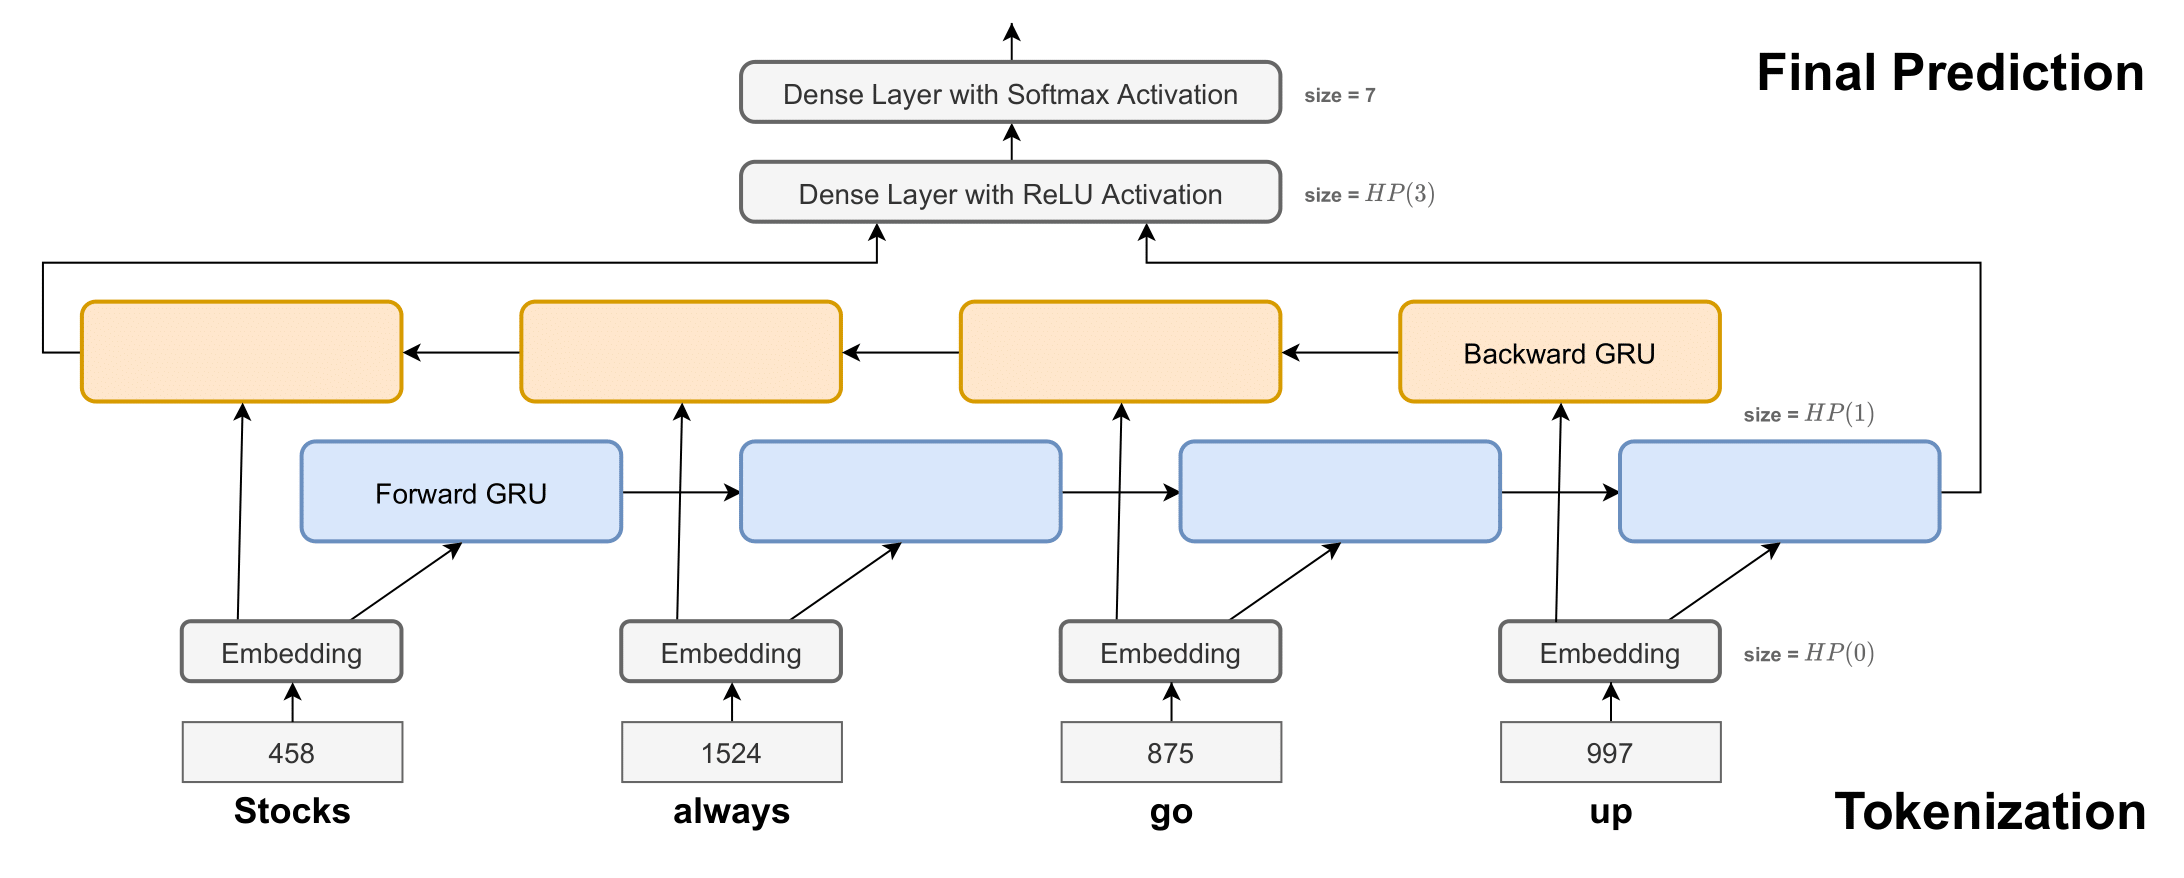
\includegraphics[width=\textwidth,height=\textheight,keepaspectratio]{architecture.drawio.png}

\noindent The model contains three essential subparts: the embedding layer, the bidirectional GRU layers, and the final densely connected layers. Each layer has one or more hyperparameters (denoted by $HP(i)$) that are subject to tuning. Documents are fed into the model in the form of tokens identified from the encoder. There are 16,003 unique tokens identified in the training data. The embedding layer is a neural net that converts each token into a vector of length $HP(0)$. These embedded vectors are then received as input by the two GRU layers. GRU are a form of recurrent neural networks that use gates to better pass long term memory than simple recurrent neural nets (RNN), but have fewer parameters than long short-term memory (LSTM) neural nets. This allows for GRUs to be more expressive than simple RNNs faster and easier to train than LSTMs. Research also suggest that performance of GRUs are comparable with LSTMs for some natural language processing models (\cite{GRU}). GRU also do not differentiate between the output and hidden vectors and the sizes of these hidden vectors are $HP(1)$. The final hidden vectors of both GRUs (forward and backward) are then concatenated and fed into a dropout layer with dropout rate $HP(2)$ followed by a densely connected network of two layers separated by another dropout layer with the same rate of $HP(2)$. These two dense layers are of size $HP(3)$ and 7 with ReLU and Softmax activation functions respectively. All training is done using the Adam Optimizer.

\subsubsection{Training Process}
In this project, we have trained three discriminative models that are compared and evaluated. These are:
\begin{enumerate}
\itemsep0pt
  \item Neural network trained only on synthetic data generated by the LDA generative model
  \item Neural network trained on synthetic data with continued training on real data
  \item Neural network trained only on real data
\end{enumerate}

\noindent TODO: Learning rate range test: final learning rate: 10\textsuperscript{-2.5}



\noindent We begin by tuning the models hyperparameters on the synthetic data set. The tuning is implemented using the optuna library (\cite{optunapaper}) and its implementation of Tree-structured Parzen Estimators, a sequential model-based optimization approach to intelligently exploring hyperparameter search spaces (\cite{bergstraTPE}). Each experiment is run for 50 trials (1 trial = one entire training run) due to time constraints. Each model is trained for 20 epochs, but we employ an early stopping mechanisms to stop training after 3 epochs without validation accuracy increase as, empirically, our models converged quickly and performance plateaued. The batch size for our experiments is fixed at 64.

\begin{center}
\begin{tabular}{llc}
\toprule
    Parameter & Description & Search Space \\
\midrule
    HP(0) & Embedding dim & $\{16k \vert k\in \{1, 2, 3, 4, 5\}\}$\\
    HP(1) & GRU dim & $\{16k \vert k \in \{2, 3, ..., 16\}\}$\\
    HP(2) & Dropout rate & $[0, 0.5]$\\
    HP(3) & Dense dim &  $\{16k \vert k \in \{1, 2, ..., 16\}\}$\\
    HP(4) & $\ell_2$ regularization & $[10\mathrm{e}^{-9}, 0.5]$ \\
\bottomrule
\end{tabular}
\end{center}
\begin{center}
	Table X: Hyperparameters and their search spaces.
\end{center}

\noindent After finding the optimal hyperparameter configuration (shown in Table XX), we refit the model using the optimal parameters and benchmark its performance on the synthetic and real data. Subsequently, we continue training the same model on the real data set. We hypothesize that pre-training on synthetic data might help the model converge faster on real-world data. After training for another 20 epochs, we benchmark the model again.

\noindent To gauge whether pre-training on synthetic data had an impact on model performance or training behavior, we conduct another experiment. We start a new hyperparameter search with the same model architecture and search space, but this time on the real data set. We use the optimal parameters to create a third neural network model that has never seen synthetic data and benchmark it on both, the synthetic and real test set. Table XX shows the optimal parameter configurations found in each run.


\begin{center}
\begin{tabular}{llcc}
\toprule
    Parameter & Description & Synthetic Data & Real Data \\
\midrule
    HP(0) & Embedding dim & 32 & 64\\
    HP(1) & GRU dim & 64 & 48\\
    HP(2) & Dropout rate & 0.1 & 0.25\\
    HP(3) & Dense dim & 64 & 112\\
    HP(4) & $\ell_2$ regularization & $10\mathrm{e}^{-9}$ & $2\mathrm{e}{-8}$\\
\bottomrule
\end{tabular}
\end{center}
\begin{center}
	Table XX: Optimal hyperparameter configuration for models on synthetic and real data
\end{center}




% --------------------------------------------------------------------------------
\section{Results}
\subsection{LDA Model}

The LDA model performs exceptionally well scoring precision and recall values of around 0.98 on synthetic data. This is to be expected, as the model itself generated the data. Therefore, there is only a small amount of randomness from the sampling procedure that prevents the model from achieving an accuracy of 100\%. However, applying the same model to real-world data reveals that this performance does not translate well. The topics \texttt{thanksgiving} and \texttt{covid19} in particular seem to be hard to classify by the model as they have the lowest precision and recall values of all topics. The topic \texttt{formula1}, on the other hand, seems to be the easiest to classify, as around 55.8\% of the models \texttt{formula1} predictions are correct (precision) and the model is able to identify more than half of the \texttt{formula1} related tweets (recall = 0.562). This model achieves an accuracy of $\approx 98\%$ on synthetic and $\approx 34\%$ on real data.
\begin{center}
\begin{tabular}{lrrrr}
\toprule
{} &  precision &  recall &  f1-score &  support \\
\midrule
thanksgiving    &      0.946 &   0.979 &     0.962 &     2000 \\
formula1        &      0.986 &   0.977 &     0.982 &     1942 \\
covid           &      0.986 &   0.986 &     0.986 &     1976 \\
championsleague &      0.986 &   0.969 &     0.977 &     2092 \\
crypto          &      0.986 &   0.987 &     0.987 &     2014 \\
tesla           &      0.986 &   0.976 &     0.981 &     2054 \\
holidays        &      0.967 &   0.969 &     0.968 &     1922 \\
\bottomrule
\end{tabular}

\qquad
\begin{tabular}{lrrrr}
\toprule
{} &  precision &  recall &  f1-score &  support \\
\midrule
thanksgiving    &      0.150 &   0.107 &     0.125 &     2122 \\
formula1        &      0.558 &   0.562 &     0.560 &     1975 \\
covid           &      0.034 &   0.022 &     0.026 &     2026 \\
championsleague &      0.339 &   0.443 &     0.384 &     1541 \\
crypto          &      0.333 &   0.304 &     0.318 &     1988 \\
tesla           &      0.412 &   0.319 &     0.359 &     2021 \\
holidays        &      0.387 &   0.670 &     0.490 &     1996 \\
\bottomrule
\end{tabular}

\end{center}
\begin{center}
Table 1 \& 2: Benchmark results of LDA model on synthetic data (left) and real data (right)
\end{center}

\subsection{Neural Networks}
\subsubsection{Training on Synthetic Data Only}
The neural network trained on synthetic data is almost able to achieve the same performance metrics as the LDA model, although it performs slightly worse for almost every topic. The generalization to real data, however, performs slightly better than the LDA, although it is noticeable that \texttt{formula1} and \texttt{holidays} seem to be the hardest topics to classify.
The model achieves an accuracy of $\approx 95\%$ on synthetic and $\approx 35\%$ on real data.

\begin{center}
\begin{tabular}{lrrrr}
\toprule
{} &  precision &  recall &  f1-score &  support \\
\midrule
thanksgiving    &      0.503 &   0.515 &     0.509 &     2046 \\
formula1        &      0.024 &   0.031 &     0.027 &     1512 \\
covid           &      0.734 &   0.467 &     0.571 &     3162 \\
championsleague &      0.866 &   0.670 &     0.755 &     2509 \\
crypto          &      0.596 &   0.691 &     0.640 &     1656 \\
tesla           &      0.765 &   0.675 &     0.717 &     2329 \\
holidays        &      0.094 &   0.238 &     0.134 &      786 \\
\bottomrule
\caption{Benchmark results of neural net (trained on synthetic data only) on synthetic data}
\end{tabular}
	
\qquad
\begin{tabular}{lrr}
\toprule
{} &  precision &  recall \\
\midrule
thanksgiving    &      0.499 &   0.401 \\
formula1        &      0.033 &   0.037 \\
covid19         &      0.183 &   0.454 \\
championsleague &      0.484 &   0.503 \\
crypto          &      0.717 &   0.317 \\
tesla           &      0.326 &   0.495 \\
holidays        &      0.099 &   0.150 \\
\bottomrule
\end{tabular}

\end{center}
\begin{center}
Table 3 \& 4: Benchmark results of neural net (trained on synthetic data only) on synthetic data (left) and real data (right)
\end{center}




\subsubsection{Training on Synthetic Data and Real Data}
Next, we assess the predictive performance of a model that has been trained on the synthetic data set first, and then continues training on the real data set. While its performance on the synthetic data after finishing the training is worse than the models discussed before, it outperforms them on the real data set achieving consistently good performance across all topics. The model achieves an accuracy of $\approx 51\%$ on synthetic and $\approx 83\%$ on real data.
\begin{center}
\begin{tabular}{lrr}
\toprule
{} &  precision &  recall \\
\midrule
thanksgiving    &      0.386 &   0.524 \\
formula1        &      0.009 &   0.012 \\
covid19         &      0.797 &   0.518 \\
championsleague &      0.857 &   0.542 \\
crypto          &      0.543 &   0.751 \\
tesla           &      0.838 &   0.567 \\
holidays        &      0.032 &   0.164 \\
\bottomrule
\end{tabular}

\qquad
\begin{tabular}{lrr}
\toprule
{} &  precision &  recall \\
\midrule
thanksgiving    &      0.883 &   0.830 \\
formula1        &      0.791 &   0.890 \\
covid19         &      0.840 &   0.809 \\
championsleague &      0.861 &   0.783 \\
crypto          &      0.815 &   0.773 \\
tesla           &      0.777 &   0.812 \\
holidays        &      0.880 &   0.955 \\
\bottomrule
\end{tabular}
% Accuracy: 0.8337844758212013
\end{center}
\begin{center}
Table 3 \& 4: Benchmark results of neural net (trained on synthetic data 

and real data) on synthetic data (left) and real data (right)
\end{center}


\subsubsection{Training on Real Data Only}
The model achieves an accuracy of $\approx 42\%$ on synthetic and $\approx 84\%$ on real data.
\begin{center}
\begin{tabular}{lrr}
\toprule
{} &  precision &  recall \\
\midrule
thanksgiving    &      0.395 &   0.482 \\
formula1        &      0.052 &   0.046 \\
covid19         &      0.519 &   0.350 \\
championsleague &      0.616 &   0.708 \\
crypto          &      0.566 &   0.553 \\
tesla           &      0.636 &   0.546 \\
holidays        &      0.048 &   0.092 \\
\bottomrule
\end{tabular}

\qquad
\begin{tabular}{lrr}
\toprule
{} &  precision &  recall \\
\midrule
thanksgiving    &      0.885 &   0.822 \\
formula1        &      0.825 &   0.810 \\
covid19         &      0.865 &   0.769 \\
championsleague &      0.796 &   0.844 \\
crypto          &      0.862 &   0.710 \\
tesla           &      0.680 &   0.855 \\
holidays        &      0.838 &   0.979 \\
\bottomrule
\end{tabular}

\end{center}
\begin{center}
Table 5 \& 6: Benchmark results of neural net (trained on real data only)

 on synthetic data (left) and real data (right)
\end{center}


\subsection{A Look at the Learned Word Embeddings}
To verify that the neural network model has learned meaningful word embeddings, we feed it seven manually chosen words (one closely related to each topic, but never the name of the topic itself) and find the ten closest word in the embedding space using cosine similarity. We find that the word embeddings capture an impressive amount of meaning: The name of Formula 1 driver Lewis Hamilton is closest to other drivers' names as well as ``formula" and ``race". ``Barcelona" maps to other sports clubs that plays in the Champions League. Similarly,  we observe that ``vaccine" is close to health- and covid-related words while ``Christmas" is similar to ``December" and ``festive". For ``Elon" and ``BTC" the closest words are coherent and refer to Tesla and Cryptocurrencies. Only ``turkey" is not clearly close to Thanksgiving, presumably as the topic \texttt{thanksgiving} has been hard to identify throughout the experiments. It is interesting to note that various relevant emojis have been identified as closely-related to each topic word, which confirms our initial hypothesis that emojis can be as meaningful as other words.
\\

\begin{adjustbox}{width=\columnwidth,center}
\begin{tabular}{lllllll}
\toprule
    hamilton &   barcelona &     vaccine & christmas &     turkey &         elon &         btc \\
\midrule
         max & bayernbarça &    immunity &  december &          🦃 &         musk &     cryptos \\
        ocon &           ⚽ &    vaccines &  nicholas &       nick &          fsd &       coins \\
       lewis &       zenit &      deaths &   festive &     cotton &       teslas &         eth \\
         vsc &       barca &       tests &     visit &       flex &           ev &      ssfeed \\
championship &      bayern &    measures &   snowman &  gratitude & supercharger &      tether \\
         abu &         ucl &       boris &      pack &        nov &      binance &          io \\
         fia &   liverpool &     booster &    wreath &   rosemary &    cointrade & opportunity \\
     formula &       milan &  vaccinated &   rainbow & chronicles &         giga &        dump \\
        race &    matchday & vaccination &         🥃 &  skyrocket &    autopilot &   analyzing \\
\bottomrule
\end{tabular}

\end{adjustbox}
\begin{center}
	Table 9: Top 10 closest words in embedding space for seven examples.
\end{center}

% --------------------------------------------------------------------------------
\section{Discussion}
- NN synthonly \& LDA super similar (with same bad generalization)
- Synthandreal \& realonly have similar real world performance
- F1 and holiday seem to be different between synth data and real data (good acc on real data but bad on synth data)

% Mention catastrophic forgetting:
While performing better on real data, the network that is trained on synthetic data first and then continues learning on real data has an inferior performance on synthetic data compared to all other models that were trained on the synthetic data set. Apparently, continuing training on real data makes the model un-learn relationships in the artificial data set. This phenomenon is known as \emph{Catastrophic Forgetting} and is an ongoing area of research (e.g. \cite{kaushik2021understanding}). We have to add that for our example, the results indicate that the artificially generated data set and real data set seem to be slightly dissimilar. This can be partly explained by the LDA being a bag-of-words model and therefore not generation sequential data. Moreover, we manually had to label the inferred topics, which worked well for the majority of topics, but turned out to not perfectly recreate the topics \texttt{covid19} and \texttt{thanksgiving}.


% --------------------------------------------------------------------------------
\section{Conclusion}


% --------------------------------------------------------------------------------
\newpage
\printbibliography

\end{document}
